El módulo de bajo consumo es el encargado de reducir el consumo del sistema cuando no es necesario que funcione a plena potencia, es decir, entre las obtenciones de las diferentes medidas.


Las librerías incluidas con el ESP8266 incluye un modo de bajo consumo ya definido llamado deep-sleep, el cual desactiva el WIFI, el reloj del sistema y la CPU, es decir, solo mantiene el funcionamiento del RTC y reduce el consumo del sistema a apenas unas decenas de micro amperios. Sin embargo, debido a que este modo de bajo consumo inhabilita también los GPIOs es incompatible con nuestro sistema ya que, si se activara, el proyecto quedaría inutilizado completamente. Debido a esto, este modo de bajo consumo no es apto para nuestro sistema.
\todo[inline]{citar Bajo Consumo}

\begin{figure}[H]
    \centering
    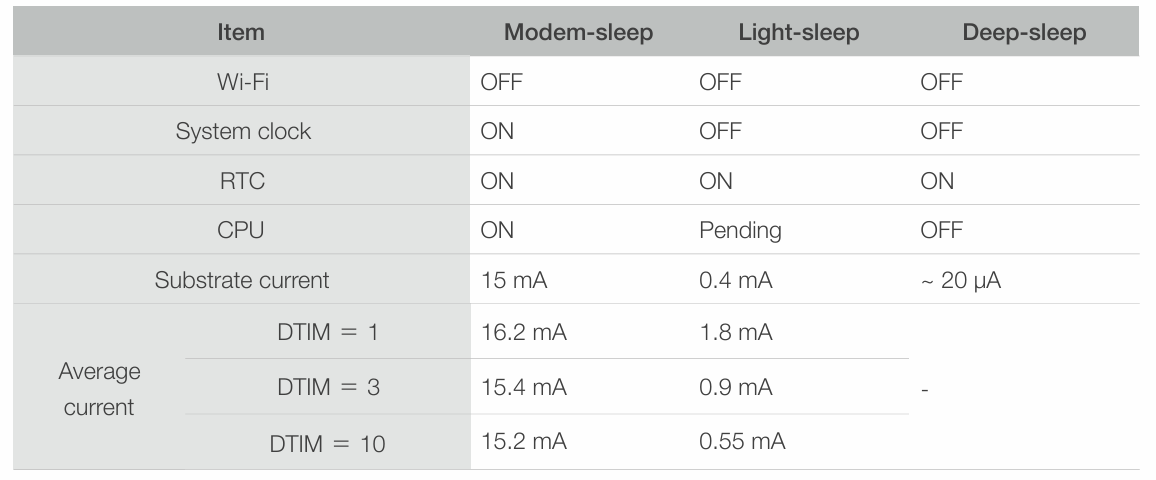
\includegraphics[width=0.6\textwidth]{images/3-software/3-2-5-lowpower/Modos Bajo Consumo.png}
    \caption{Modos Bajo Consumo ESP8266}
    \label{fig:3-2-5-1-ModosBajoConsumo}
\end{figure}

Debido a este requisito, hemos desarrollado nuestro propio modo de bajo consumo, el cual reduce el consumo del sistema en un 80\% aproximadamente. Este modo de bajo consumo es similar al llamado modem-sleep. Por nuestra parte, nuestro modo desactiva el wifi, baja la frecuencia del reloj del sistema y ejecuta un delay, para que el micro reduzca su consumo. Debido a que en ningún momento se inhabilitan los GPIOs, este modo de bajo consumo es perfecto para nuestro sistema.


Este módulo esta dividido en dos ficheros, \texttt{sleep.hpp} el cual contiene la definición de la función de bajo consumo y la importación de la librería necesaria, y el fichero \texttt{sleep.cpp}, el cual contiene la implementación de dicha función, que recibe como parámetro el tiempo en milisegundos deseado de duración del modo de bajo consumo y no devuelve nada.

\begin{lstlisting}[captionpos=b, caption={Función bajo consumo}, language=c++]
    void sleep_low_power(int time_delay) {}
\end{lstlisting}

La secuencia de ejecución se puede dicir en dos secuencias consecutivas, una que activa el modo de bajo consumo y otra que restaura el funcionamiento normal. La secuencia de activación es la siguiente:

\begin{enumerate}
    \item Se desactiva el módulo de WIFI, activando el modo \texttt{WIFI\_OFF}.
    \item Se llama a la función \texttt{forceSleepBegin()}, la cual guarda el modo de WIFI actual y fuerza el estado de modem sleep del WIFI, reduciendo aún más el consumo.
    \item Se reduce frecuencia del reloj del sistema a la mínim valor posible, 80 MHZ.
    \item Se introduce un delay. Esto asegura que el microprocesador consumirá menos durante dicho tiempo, además se utiliza para definir la duración aproximada del modo de bajo consumo.
\end{enumerate}

\begin{lstlisting}[captionpos=b, caption={Activación modo bajo consumo}, language=c++]
    Serial.println("[SLEEP] Entrando en modo bajo consumo");
    WiFi.mode(WIFI_OFF);
    WiFi.forceSleepBegin();
    system_update_cpu_freq(SYS_CPU_80MHZ);

    delay(time_delay);
\end{lstlisting}

Una vez pasado el tiempo definido de bajo consumo, se entra en la secuencia de restauración, la cual consta de los siguientes pasos:

\begin{enumerate}
    \item Aumentar la frecuencia del reloj al valor anterior, 160 MHz.
    \item Forzar la activación del módulo del WIFI.
    \item Aplicar un delay de 1 ms para asegurar que el módulo WIFI se haya despertado.
    \item Configurar el módulo de WIFI como una estación, es decir, configurar el ESP8266 como un dispositivo que se conecta a un punto de acceso.
\end{enumerate}

\begin{lstlisting}[captionpos=b, caption={Restauración modo bajo consumo}, language=c++]
    Serial.println("[SLEEP] Saliendo del modo bajo consumo");
    system_update_cpu_freq(SYS_CPU_160MHZ);
    WiFi.forceSleepWake();
    delay(1);
    WiFi.mode(WIFI_STA);
\end{lstlisting}

Mediante la implementación de nuestro propio modo de bajo consumo, nos aseguramos que correcto funcionamiento durante y después de dicho modo, reduciendo el consumo del sistema un 80\% aproximadamente.